\chapter{Cubical grids and topological products}

%--------------------------------------------------------------------------------
\subsection{Summary}
%--------------------------------------------------------------------------------

Here we introduce a fast implementation of the general Cartesian product of cellular complexes. Both kind of operators, depending on the dimension of their input, may generate either full-dimensional (i.e.~solid) output complexes or cellular complexes of dimension $d$ embedded in Euclidean space of dimension $n$, with $d\leq n$. 

%++++++++++++++++++++++++++++++++++++++++++++++++++++++++++++++++++++++++++++++++
\section{Introduction}
%++++++++++++++++++++++++++++++++++++++++++++++++++++++++++++++++++++++++++++++++
This chapter aims to discuss the design and the implementation of the \texttt{largrid} module of the \texttt{LARLIB.jl} library, including also the Cartesian product of general cellular complexes. 
In particular, we show that both $n$-dimensional grids of (hyper)-cuboidal cells and their  $d$-dimensional skeletons ($0\leq d\leq n$), embedded in $\E^n$, may be properly and efficiently generated by assembling the cells produced by a number $n$ of either $0$- or $1$-dimensional cell complexes, that in such lowest dimensions coincide with simplicial complexes. 

In Section~\ref{sec:0-1-complexes} we give the simple implementation of generation of lower-dimensional (say, either 0- or 1-dimensional) regular cellular complexes with integer coordinates.
In Section~\ref{sec:cuboids} a functional decomposition of the generation of either full-dimensional cuboidal complexes in $\E^n$ and of their $d$-skeletons ($0\leq d\leq n$) is given, showing in particular that every skeleton can be efficiently generated as a partition in cell subsets produced by the Cartesian product of a proper disposition of 0-1 complexes, according to the binary representation of a subset of the integer interval $[0,2^n]$.

In Section~\ref{sec:product} we provide a very simple and general implementation of the topological product of \emph{two} cellular complexes of any topology. When applied to embedded linear cellular complexes (i.e.~when the coordinates of 0-cells of arguments are fixed and given) the algorithm produces a Cartesian product of its two arguments.
In Section~\ref{sec:largrid} the exporting of the module to different languages is provided.

The Section~\ref{sec:tests} contains the unit tests associated to the various algorithms, that are exported by the used literate environment in the proper test subdirectory---depending on the implementation language.
In Section~\ref{sec:indices} the indexing structure of the macro sources and variables is exposed by the sake of the reader. 
The Appendix~\ref{sec:utilities} contains some programming utilities possibly needed by the developers.


\section{0D- and 1D-complexes}
\label{sec:0-1-complexes}

%++++++++++++++++++++++++++++++++++++++++++++++++++++++++++++++++++++++++++++++++
\section{Implementation}
%++++++++++++++++++++++++++++++++++++++++++++++++++++++++++++++++++++++++++++++++

\subsection{Largrid exporting}
\label{sec:largrid}
We assemble top-down the \texttt{largrid.jl} file, by listing the macros it is composed of. 
As might be expected, the present one is the module version corresponding to the current state of the system, i.e.~to a very initial state.
%------------------------------------------------------------------
@O lib/jl/largrid.jl
@{
#= Functions for grid generation and Cartesian product =#

using IterTools
using DataStructures

@< Generation of uniform 0D cellular complex  @>
@< Generation of uniform 1D cellular complex  @>
@< Generation of cellular complex of dimension $d = 0 | 1$ @>
@< Generation of grid vertices  @>
@< Transformation from multindex to address in a linear array storage @>
@< Generation of grid cells  @>
@< Enumeration of binary ranges of given order @>
@< Filtering binary ranges by order @>
@< Assembling grid skeletons @>
@< Multidimensional grid generation @>
@< Cartesian product of two lar models   @>
@}
%------------------------------------------------------------------




%--------------------------------------------------------------------------------
\subsection{Generation of cells}
%--------------------------------------------------------------------------------

We are going to use 0- and 1-dimensional cell complexes as the basic material for several operations, including generation of simplicial and cellular grids and topological and Cartesian product of cell complexes. 


\paragraph{Uniform 0D complex}
The \texttt{grid0} second-order function generates a 0-dimensional uniform complex embedding $n+1$ equally-spaced (at unit intervals) 0-cells within the 1D interval. It returns the cells of this 0-complex.

%-------------------------------------------------------------------------------
@d Generation of uniform 0D cellular complex 
@{function grid_0(n)
    return hcat([[i] for i in range(0,n+1)]...)
end
@}
%-------------------------------------------------------------------------------

\paragraph{Uniform 1D complex}
A similar \texttt{grid1} function returns a uniform 1D cellular complex with $n$ 1D \texttt{cells}.

%-------------------------------------------------------------------------------
@d Generation of uniform 1D cellular complex 
@{function grid_1(n)
    return hcat([[i,i+1] for i in range(0,n)]...)
end
@}
%-------------------------------------------------------------------------------

\paragraph{Uniform 0D or 1D complex}
A \texttt{larGrid} function is finally given to generate the LAR representation of the cells of either a 0- or a 1-dimensional complex, depending on the value of the \texttt{d} parameter, to take values in the set $\{0,1\}$, and providing the \emph{order} of the output complex.
%-------------------------------------------------------------------------------
@d Generation of cellular complex of dimension $d = 0 | 1$
@{function larGrid(n)
    function larGrid1(d)
        if d==0 
        	return grid_0(n)
        elseif d==1 
        	return grid_1(n) 
        end
    end
    return larGrid1
end
@}
%-------------------------------------------------------------------------------



function cart(args)
	return sort(collect(IterTools.product(args...)))
end



%--------------------------------------------------------------------------------
\section{Cuboidal grids}\label{sec:cuboids}
%--------------------------------------------------------------------------------

More interesting is the generation of \emph{hyper-cubical grids} of intrinsic dimension $d$ embedded in $n$-dimensional space, via the Cartesian product of $d$ 1-complexes and $(n-d)$ 0-complexes. When $d=n$ the resulting grid is said \emph{solid}; when $d=0$ the output grid is 0-dimensional, and corresponds to a grid-arrangement of a discrete set of points in $\E^n$.


\subsection{Full-dimensional grids}
%--------------------------------------------------------------------------------

\subsubsection{Vertex generation}

First the grid vertices are produced by the \texttt{larVertProd} function, via Cartesian product of vertices of the $n$ 1-dimensional arguments (vertex lists in \texttt{vertLists}), orderly corresponding to $x_0$, $x_1$, ..., $x_{n-1}$ in the output points $(x_0, x_1,\ldots,x_{n-1})$.
%-------------------------------------------------------------------------------
@d Generation of grid vertices 
@{function larVertProd(vertLists)
	coords = [[x[1] for x in v] for v in cart(vertLists)]
   return sortcols(hcat(coords...))
end
@}
%-------------------------------------------------------------------------------




\subsubsection{Mapping of indices to storage}

\paragraph{Multi-index to address transformation}
The second-order utility \texttt{index2addr} function transforms a \texttt{shape} list for a multidimensional array into a function that, when applied to a multindex array, i.e.~to a list of integers within the \texttt{shape}'s bounds, returns the integer address of the array component within the linear storage of the multidimensional array.

The transformation formula for a $d$-dimensional array with \texttt{shape} $(n_0,n_1,...,n_{d-1})$ is a linear combination of the 0-based\footnote{0-based array, like in C, java and python, as opposed to 1-based, like in fortran or matlab.} multi-index $(i_0,i_1,...,i_{d-1})$ with \texttt{weights} equal to $(w_0,w_1,...,w_{d-2},1)$:
\[
addr = i_0\times w_0 +i_1\times w_1 +\cdots +i_{d-1}\times w_{d-1}
\]
where 
\[
w_k = n_{k+1} \times n_{k+2} \times\cdots\times  n_{d-1}, \qquad 0\leq k\leq d-2.
\]

Therefore, we get $\texttt{index2addr([4,3,6])([2,2,0])}=48= 2\times(3\times 6)+2\times(6\times 1)+0$,
where \texttt{[2,2,0]} represent the numbers of (pages, rows, columns) indexing an element in the three-dimensional array of shape \texttt{[4,3,6]}.

%-------------------------------------------------------------------------------
@d Transformation from multindex to address in a linear array storage
@{function index2addr(shape::Array{Int64,1})
	index2addr(hcat(shape...))
end

function index2addr(shape::Array{Int64,2})
    n = length(shape)
    theShape = append!(shape[2:end],1)
    weights = [prod(theShape[k:end]) for k in range(1,n)]
    function index2addr0(multiIndex)
        return dot(collect(multiIndex), weights) + 1
    end
    return index2addr0
end
@}
%-------------------------------------------------------------------------------


\subsubsection{Cartesian product of 0/1-complexes}
Here, the input is given by the array \texttt{cellLists} of lists of cells of the argument complexes. Hence, the \texttt{shapes} variable contains the (list of) numbers $m_0, m_1, ...$ of cells in each argument complex, and the \texttt{indices} variable (generated by Cartesian product) collects the whole set $M_0 \times M_1 \times \cdots$ of 0-based multi-indices corresponding to the cells of the output complex, with $M_k = \{0,1,...,m_{k}-1\}$.

The \texttt{jointCells} variable is used to contain the list of outputs of Cartesian products of \texttt{cells} corresponding to every \texttt{index} in \texttt{indices}.

%-------------------------------------------------------------------------------
@D Generation of grid cells 
@{function larCellProd(cellLists)
	shapes = [length(item) for item in cellLists]
	subscripts = cart([collect(range(0,shape)) for shape in shapes])
	indices = hcat([collect(tuple) for tuple in subscripts]...)
	jointCells = Any[]
	for h in 1:size(indices,2)
		index = indices[:,h]
		cell = hcat(cart([cells[k+1] for (k,cells) in zip(index,cellLists)])...)
		append!(jointCells,[cell])
	end
	convertIt = index2addr([ (length(cellLists[k][1]) > 1)? shape+1 : shape 
		for (k,shape) in enumerate(shapes) ])		
	[vcat(map(convertIt, jointCells[j])...) for j in 1:size(jointCells,1)]
end
@}
%-------------------------------------------------------------------------------



\subsection{Lower-dimensional grid skeletons}

In order to compute the $d$-skeletons of a $n$-dimensional cuboidal ``grid'' complex, with $0\leq d\leq n$, let us start by remarking a similarity with the generation of the boolean representation of numbers between 0 and $2^n -1$, generated as a list of strings by the \texttt{binaryRange} function, given in Section~\ref{sec:binaryRange}.

The binary representations of such numbers are in fact filtered according to the number of their ones in Section~\ref{sec:filterByOrder}, and used to generate the distinct components of different order skeletons of the assembled grid complexes in Section~\ref{sec:assembly}.

\subsubsection{Generation of skeleton components}
\label{sec:binaryRange}

The \texttt{binaryRange} function, applied to an integer $n$, returns the string representation of all binary numerals between 0 and $2^n -1$. All the strings have the same length $n$. The bits in each strings will be used to select between either a 0- or a 1-dimensional complex as generator (via a Cartesian product of complexes) of a component of an embedded grid skeleton of proper intrinsic dimension.

%-------------------------------------------------------------------------------
@D Enumeration of binary ranges of given order
@{function binaryRange(n)
	return [bin(k,n) for k in 0:2^n-1]
end
@}
%-------------------------------------------------------------------------------



\subsubsection{Filtering grid skeleton components}
\label{sec:filterByOrder}

The function \texttt{filterByOrder} is used to partition the previous binary strings into $n+1$ subsets, such that the bits into each string sum to the same number, ranging from 0 to $n$ included, respectively.

%-------------------------------------------------------------------------------
@D Filtering binary ranges by order
@{function filterByOrder(n)
	terms = [[parse(Int8,bit) for bit in convert(Array{Char,1},term)] for term in binaryRange(n)]
	return [[term for term in terms if sum(term) == k] for k in 0:n]
end
@}
%-------------------------------------------------------------------------------




\subsubsection{Assembling grid skeleton components}
\label{sec:assembly}

We are now finally able to generate the various subsets of cells of a $d$-dimensional cuboidal grid skeleton, produced respectively by the expression \texttt{larCellProd(cellLists)} for every permutation of 0- and 1-complexes, according to the partition classes of permtation of $n$ bits previously produced. To understand why this assembling step of cells is necessary, the reader should look at Figure~\ref{fig:sleletons}, where three subsets of 2-cells of the 2-skeleton, respectively generated by the bit dispositions \texttt{[[0,1,1], [1,0,1], [1,1,0]]}, are separately displayed.
Notice also that, whereas the dimension $n$ of the embedding space is implicittly provided by the \texttt{length} of the \texttt{shape} parameter, the intrinsic dimension $d$ of the skeleton to be produced must be given explicitly.

\begin{figure}[htbp] %  figure placement: here, top, bottom, or page
   \centering
   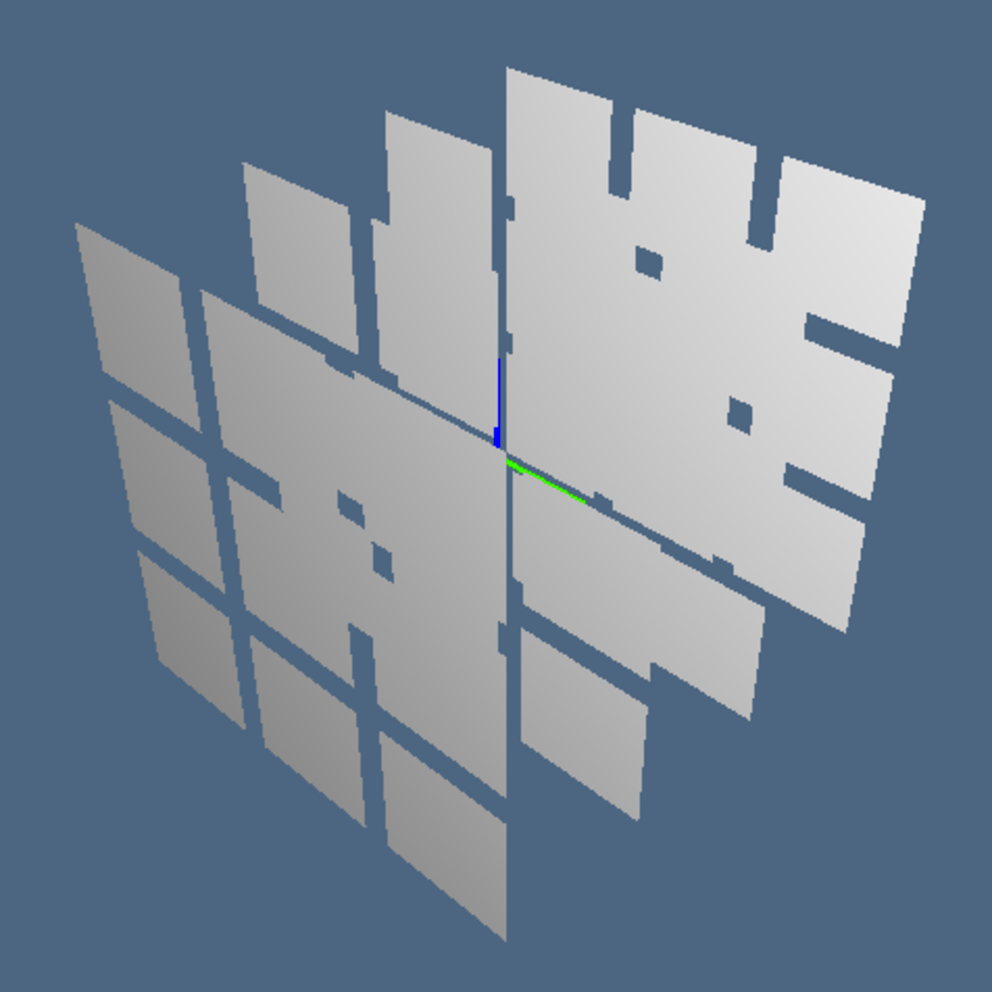
\includegraphics[height=0.245\linewidth,width=0.242\linewidth]{img/skel2a} 
   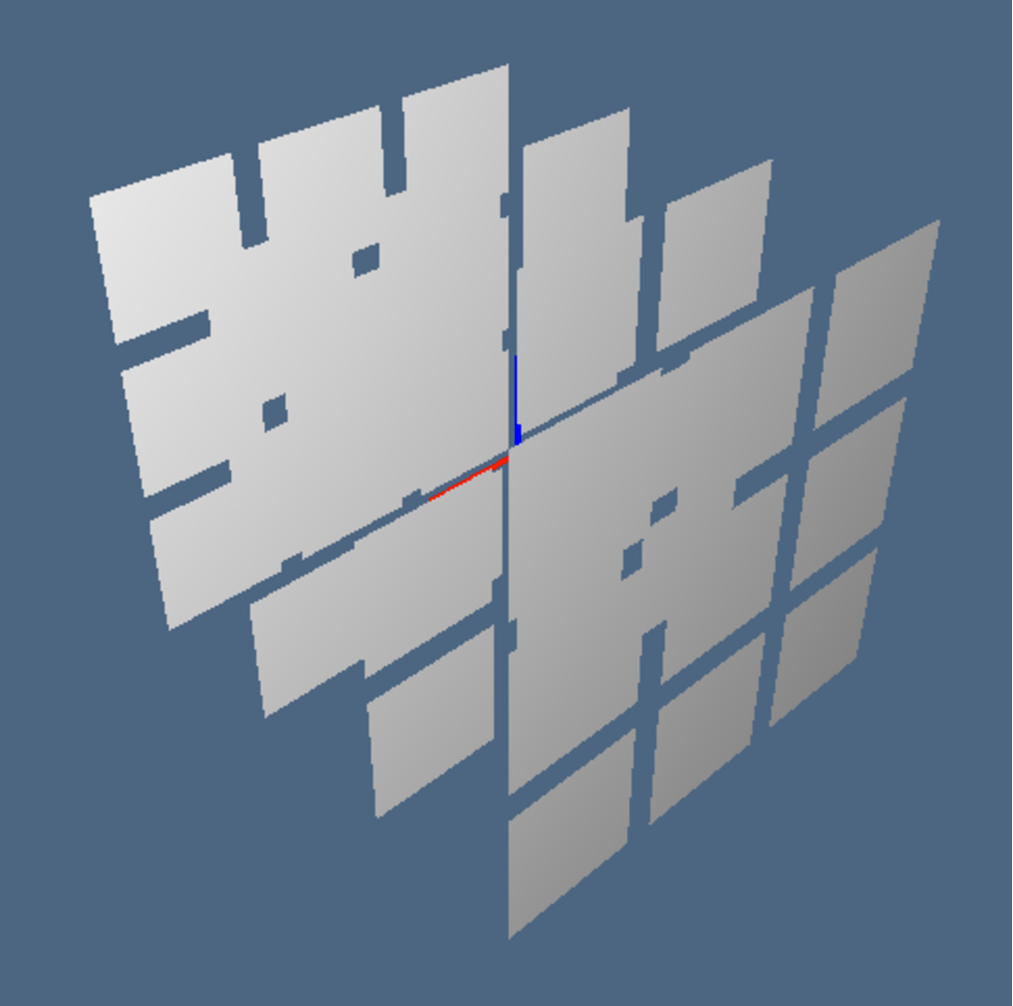
\includegraphics[height=0.245\linewidth,width=0.242\linewidth]{img/skel2b} 
   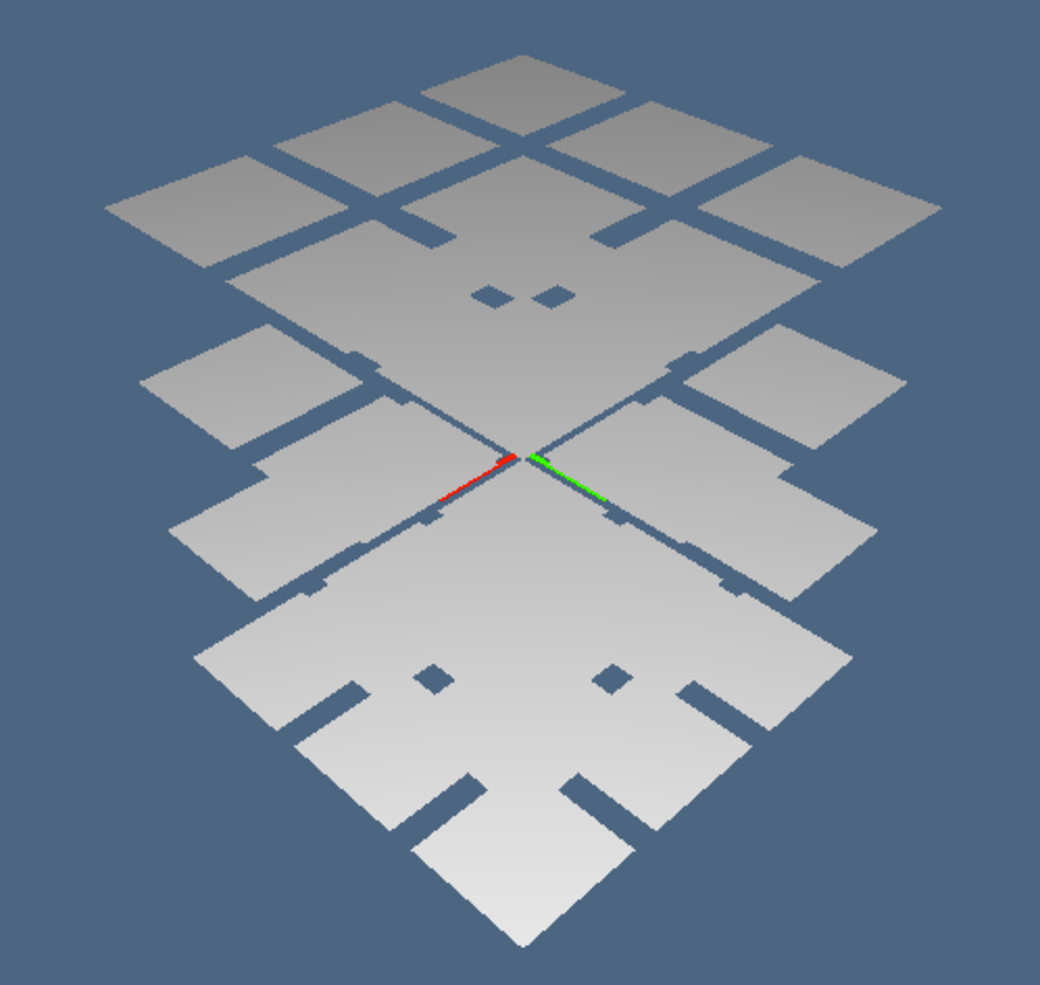
\includegraphics[height=0.245\linewidth,width=0.242\linewidth]{img/skel2c} 
   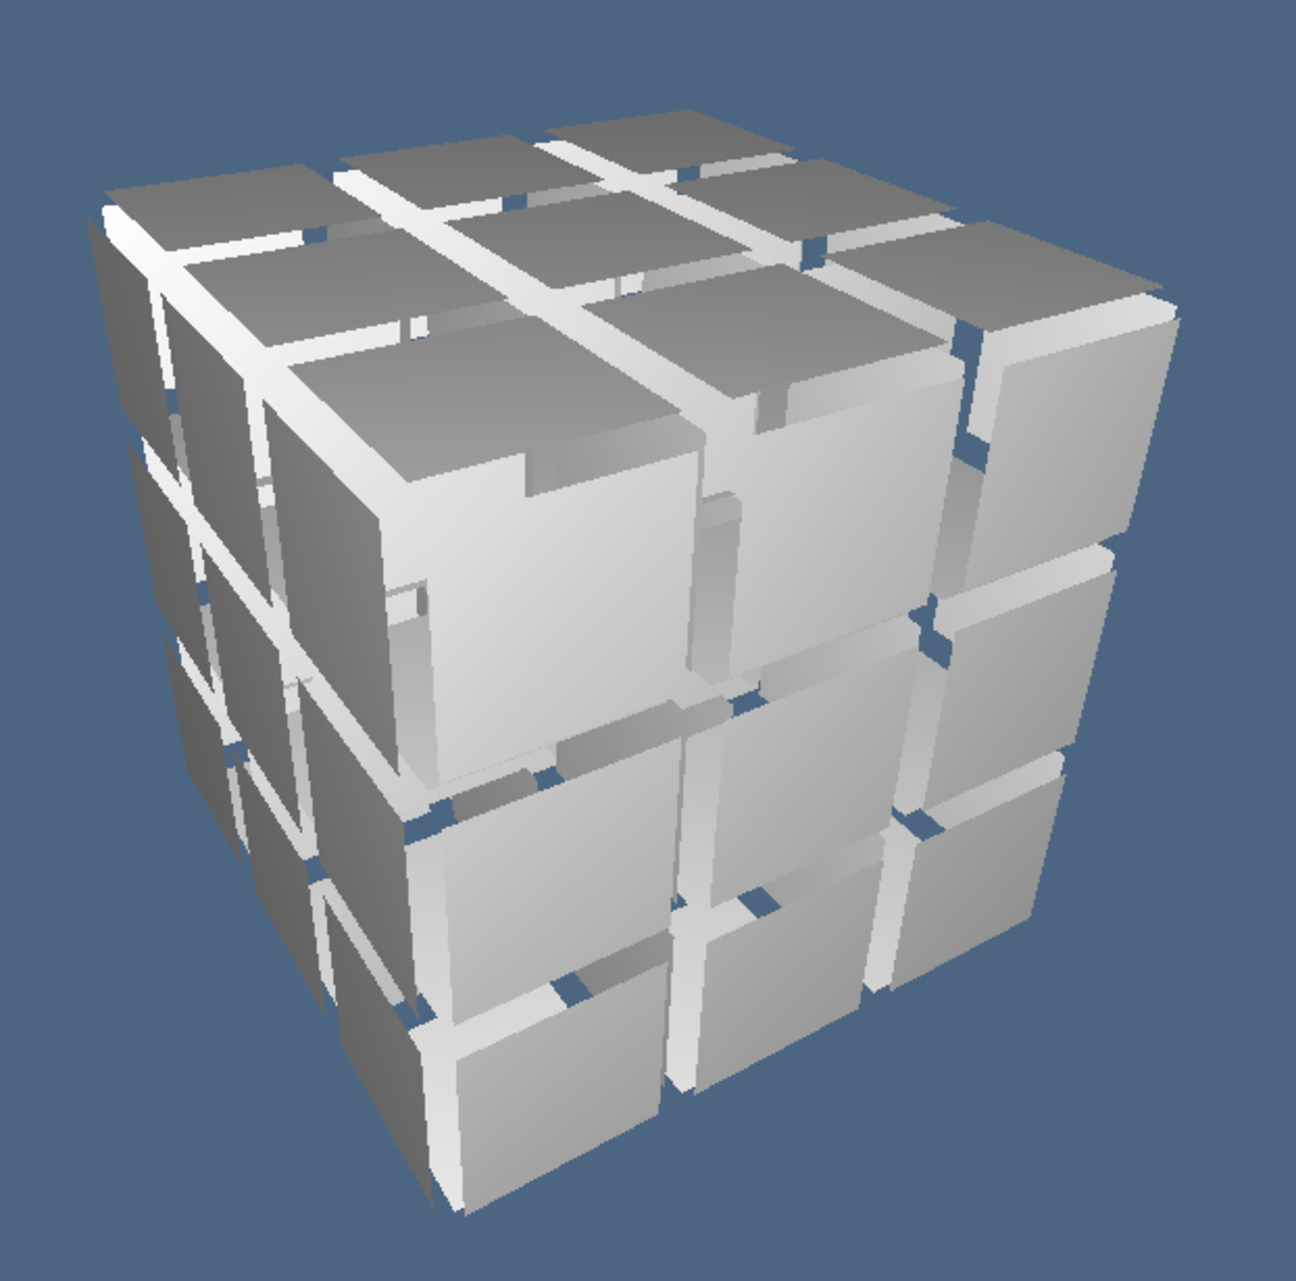
\includegraphics[height=0.245\linewidth,width=0.242\linewidth]{img/skel2} 
   \caption{(a,b,c) Exploded views of subsets (orthogonal to coordinate axes) of 2-cells of a 2-skeleton grid; (d) their assembled set.}
   \label{fig:sleletons}
\end{figure}

%-------------------------------------------------------------------------------
@D Assembling grid skeletons
@{function larGridSkeleton(shape)
    n = length(shape)
    function larGridSkeleton0(d)
        components = filterByOrder(n)[d+1]
        mymap(arr) = [arr[:,k]  for k in 1:size(arr,2)]
        componentCellLists = [ [ mymap(f(x)) for (f,x) in zip( [larGrid(dim) 
        	for dim in shape],component ) ]
            	for component in components ]
        out = [ larCellProd(cellLists)  for cellLists in componentCellLists ]
        return vcat(out...)
    end
    return larGridSkeleton0
end
@}
%-------------------------------------------------------------------------------

\subsection{Highest-level grid interface}

The highest-level user interface for (hyper)-cuboidal grid generation is given by the function \texttt{larCuboids}  applied to the \texttt{shape} parameter.  
For the sake of storage efficiency, the generated vertex coordinates are integer and 0-based in the lowest corner. The model may be properly scaled and/or translated \emph{a posteriori} when needed.

\paragraph{Generation of (hyper)-cuboidal grids}

The generated complex is always full-dimension, i.e.~\emph{solid}, and possibly includes the cells of all dimensions, depending on the Boolean value of the \texttt{full} parameter.
The grid's intrinsic dimension, as well as the dimension of its embedding space, are specified by the length of the \texttt{shape} parameter. See the examples in Figure~\ref{fig:grid23D}, but remember that the PLaSM visualiser always embed in 3D the displayed model. 

%-------------------------------------------------------------------------------
@D Multidimensional grid generation
@{function vertexDomain(n)
	return hcat([k for k in 0:n-1]...)
end

function larImageVerts(shape)
	vertLists = [vertexDomain(k+1) for k in shape]
	vertGrid = larVertProd(vertLists)
	return vertGrid
end

function larCuboids(shape, full=false)
	vertGrid = larImageVerts(shape)
	gridMap = larGridSkeleton(shape)
	if ! full
		cells = gridMap(length(shape))
	else
		skeletonIds = 0:length(shape)
		cells = [ gridMap(id) for id in skeletonIds ]
	end
	return vertGrid, cells
end
@}
%-------------------------------------------------------------------------------




shape = (3,2,1)
cubes = larCuboids(shape,true)
print(cubes)

shape = (1,1,1)
cubes = larCuboids(shape,true)
print(cubes)

shape = (10,10,10)
cubes = larCuboids(shape,true)
print(cubes)


%++++++++++++++++++++++++++++++++++++++++++++++++++++++++++++++++++++++++++++++++
\section{Cartesian product of cellular complexes} \label{sec:product}
%++++++++++++++++++++++++++++++++++++++++++++++++++++++++++++++++++++++++++++++++

\paragraph{LAR model of cellular complexes}

The external representation of a LAR model (necessarily geometrical, i.e.~embedded in some $\E^n$, in order to be possible to draw it) is a pair (\emph{geometry},\emph{topology}), where \emph{geometry} is the list of coordinates of vertices, i.e.~a two-dimensional array of numbers, where vertices are given by row, and \emph{topology} is a list of cells of fixed dimension $d$. When $d=n$ the model is \emph{solid}; otherwise  the model is some emberdded $d$-skeleton ($0\leq d <n$).

\paragraph{Binary product of cellular complexes}
The \texttt{larModelProduct} function takes as input a pair of LAR models and returns the model of their Cartesian product. Since this is a pair (\emph{geometry}, \emph{topology}), its second element returns the topological product of the input topologies.

%-------------------------------------------------------------------------------
@d Cartesian product of two lar models  
@{function larModelProduct(modelOne, modelTwo)
    (V, cells1) = modelOne
    (W, cells2) = modelTwo

    @< Cartesian product of vertices @>
    @< Topological product of cells    @>

    vertexmodel = []
    for v in keys(vertices)
        push!(vertexmodel, v)
    end
    return (vertexmodel, cells)
end

function larModelProduct(twoModels)
    modelOne, modelTwo = twoModels
    larModelProduct(modelOne, modelTwo)
end
@}
%-------------------------------------------------------------------------------

\paragraph{Cartesian product of argument vertices}
The following macro is used to generate a dictionary mapping between integer ids of new vertices and the sets $V$ and $W$ of vertices of the input complexes.

%-------------------------------------------------------------------------------
@d Cartesian product of vertices  
@{vertices = collections.OrderedDict(); 
k = 1
vertices = OrderedDict()
for v in V
    for w in W
        id = [v;w]
        if haskey(vertices, id) == false
            vertices[id] = k
            k = k + 1
        end
    end
end
@}
%-------------------------------------------------------------------------------


\paragraph{Topological product of argument vertices}
Another macro generates the cells of the topological product, represented as lists of new vertices. 

%-------------------------------------------------------------------------------
@d Topological product of cells    
@{cells = []
for c1 in cells1
    for c2 in cells2
        cell = []
        for vc in c1
            for wc in c2 
                push!(cell, vertices[[V[vc];W[wc]]] )
            end
        end
        push!(cells, cell)
    end
end
@}
%-------------------------------------------------------------------------------

